%!TEX encoding = UTF-8 Unicode
%!TEX root = ../lect-week04.tex

\ifkompendium\else

\begin{Slide}{Denna vecka: Fatta datastrukturer}
\begin{itemize}
\item Läs teori
\item Gör övning \code{data}
\item Gör lab \code{???}
\end{itemize}
\end{Slide}

\fi

%%%

\begin{Slide}{Olika sätt att skapa datastrukturer}
\begin{itemize}
\item Tupler
  \begin{itemize}
  \item samla $n$ st datavärden i element \Emph{\code{_1}}, \Emph{\code{_2}}, ...  \code{_}$n$
  \item elementen kan vara av \Alert{olika} typ
  \end{itemize}
\item Klasser   
  \begin{itemize}
  \item samlar data i \Emph{attribut} med (väl valda!) namn
  \item attributen kan vara av \Alert{olika} typ
  \item definierar även metoder som använder attributen (operationer på data)
  \end{itemize}

\item Samlingar 
  \begin{itemize}
  \item speciella klasser som samlar data i element av \Alert{samma} typ
  \item finns ofta \emph{många} färdiga \Emph{bra-att-ha-metoder} 
  \end{itemize}
\end{itemize}
\end{Slide}

\ifkompendium\else

\begin{Slide}{Vad är en tupel?}
\code{("hej", 42, math.Pi)} är en 3-tupel med typ: \code{(String, Int, Double)}
\end{Slide}

\fi


\begin{Slide}{Hierarki av samlingar i scala.collection}
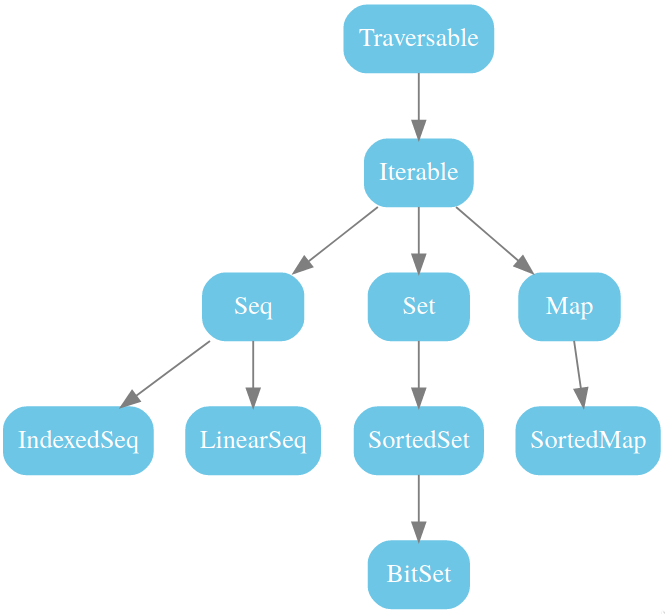
\includegraphics[width=1.0\textwidth]{../img/collection/collection-traits}
\end{Slide}

\ifkompendium
\noindent Läs mer om Scalas samlingar här: \\ 
\url{http://docs.scala-lang.org/overviews/collections/overview}
\else\fi

\ifkompendium\else

\begin{Slide}{scala.collection.immutable}
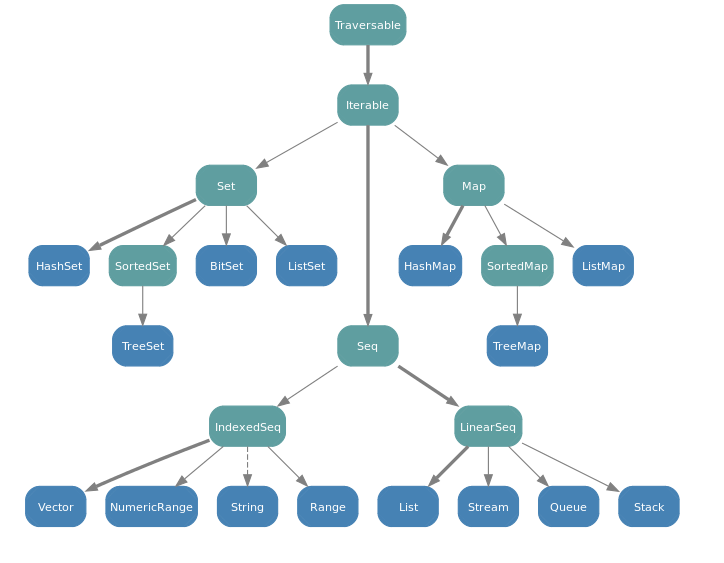
\includegraphics[width=0.82\textwidth]{../img/collection/collection-immutable}
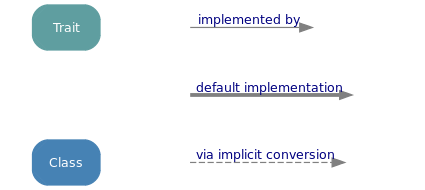
\includegraphics[width=0.33\textwidth]{../img/collection/collection-legend}
\end{Slide}

\begin{Slide}{scala.collection.mutable}
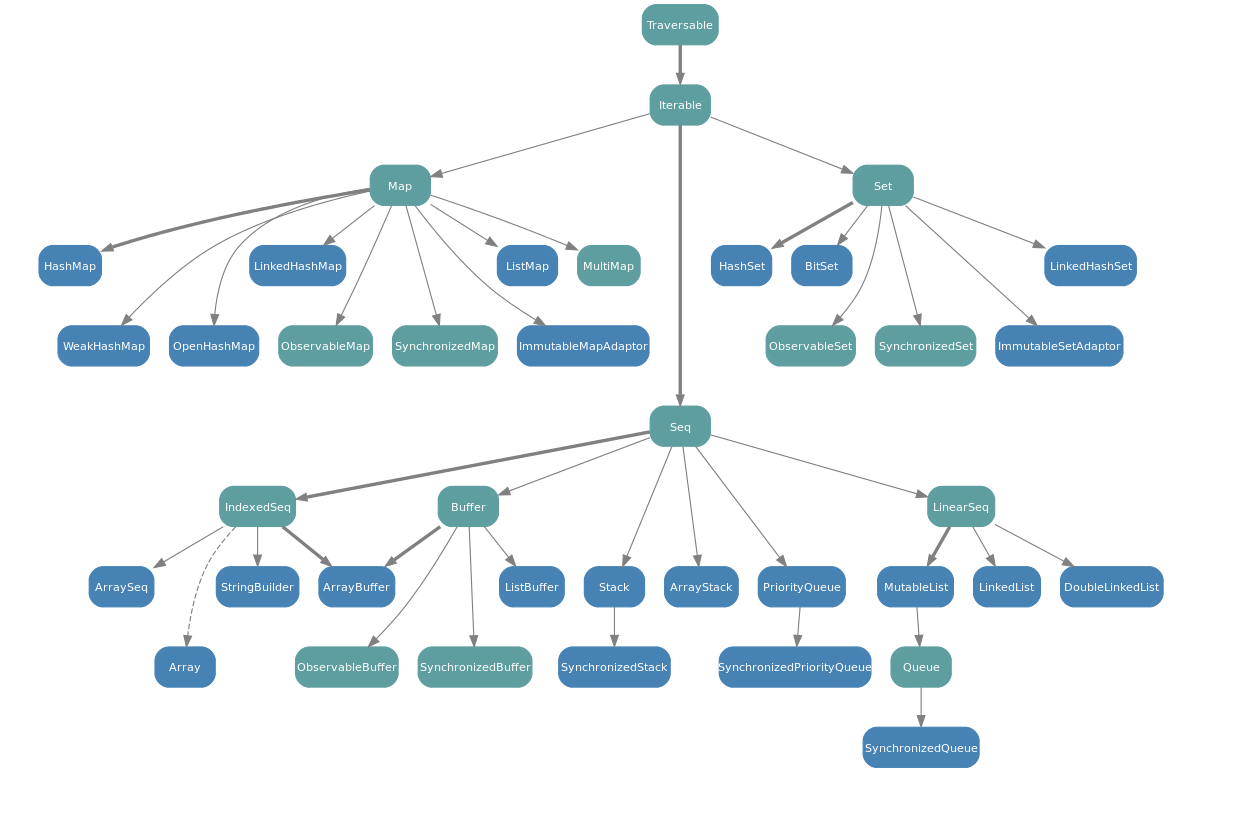
\includegraphics[width=1.05\textwidth]{../img/collection/collection-mutable}
\end{Slide}
\fi


% ??? Berätta om javafx.util.pair
% http://stackoverflow.com/questions/521171/a-java-collection-of-value-pairs-tuples



